\chapter{Precision characterisation of a Feshbach Resonance}
\label{Chap_Feshbach}

% epigraph (done: 2021年8月19日13:15:22)
\setlength{\unitlength}{1pt}
\setlength{\epigraphwidth}{11.5cm}
\epigraph{In physical science a first essential step in the direction of learning any subject is to find principles of numerical reckoning and methods for practicably measuring some quality connected with it. \cite{thomson_2011}}{--- William Thomson, 1st Baron Kelvin \\ \textit{Electrical Units of Measurement (1883)}}

\section{Overview}
% Introduction and purpose (done: 2021年8月19日13:19:11)
This chapter presents our precision calibration of a Na-Rb Feshbach resonance at 347.64 G. The purpose of inserting this chapter before discussing the droplet experiment is to require a precision map of the scattering length (actually not only Na-Rb but also Na-Na and Rb-Rb) as a function of the magnetic field. This narrative order is convenient for discussing the droplet experiment; however, the research in chronological order is tortuous as described in Sec. \ref{sec:intro-overview}. I learned my lesson that one should not trust any unverified data.

% History (done: 2021年8月19日13:24:39)
Previous measurements of Feshbach resonance(FR) parameters of Na and Rb, by three-body-loss (3B-loss) spectrum or associating method, both encountered intrinsic systematic errors, such as thermal averaging or shifting \cite{Bartenstein2005, Zurn2013}. Due to the exponential sensitivity of the droplet phase diagram, we need the scattering length map as accurate as possible. So, we implemented the dissociation method to refine the results of FR parameters at 347.64 G resonance. In the rest of this section, we will introduce what Feshbach resonance (FR) is, discuss the previous measurement results, and finally offer the arrangement of this chapter.

% what is a FR and why use FR (done: 2021年8月13日12:45:54)
Feshbach resonance as a powerful toolbox plays its essential role in cold atom experiments. With this nob, we can tune the interaction between atoms by applying an external field. Thus, it is used to explore the few-body (or many-body) physics and form molecules that open a new field in ultracold physics. Feshbach resonance requires two channels to couple to each other. One is the open channel (or entrance channel), with which collision can produce atoms, i.e. the energy of the collision pair is larger than the asymptotic energy of the channel. Another is the closed channel which offers bound states with the set energy instead of scattering state\cite{RevModPhys.82.1225}. When the energy of one bound state in the closed channel approaching the open channel threshold (typically set to be 0), the resonance happens. Near the resonance $B_0$, the two-body scattering length is approximate as
\begin{equation}
a(B) = a_{\rm bg}\left(1+\frac{\Delta}{B-B_0}\right),
\label{FR}
\end{equation}
where $a_{\rm bg}$ is the slowly varying background scattering length, and $\Delta$ is the resonance width. By simply scanning the magnetic field, the scattering length $a$ and thus the effective two-body contact interaction can be changed from repulsive (for $a > 0$) to attractive (for $a < 0$). The capability of manipulating the interaction strengths has been playing a vital role in the study of exotic physics such as the controlled collapse~\cite{donley2001}~or soliton formation in Bose-Einstein condensates (BEC)~\cite{Khaykovich2002,Strecker2002}, the BEC-BCS crossover in quantum-degenerate Fermi gases~\citep{PhysRevLett.92.040403,PhysRevLett.92.120403,Bartenstein2004,Bourdel2004}, and more recently the formation of dilute quantum droplets~\cite{petrov2015,ferrier2016Observation,cabrera2018quantum}. In addition, FRs are used to associate atomic pairs and form weakly bound Feshbach molecules (FMs)~\cite{Kohler2006}. Combined with a subsequent two-photon Raman process, this has led to the creation of long-sought ultracold ground-state molecules~\cite{ni2008,Takekoshi2014,Molony2014,Park2015,Guo2016,Voges2020}.

% Na-Rb FR previous measurements (done 2021年8月19日13:50:52)
The typical way of tuning the scattering length by an FR in the cold atom experiment is to control the magnetic field. When the magnetic field is tuned to the vicinity of the resonance, we have a large scattering length, thus can increase the two-body collision rate. This method enables us to enhance the three-body loss rate \cite{wang2013observation}, and by scanning the magnetic field, we can obtain a loss dip (as shown in Fig. \ref{FR_loss}). This phenomenon can be used to characterize an FR directly at first glance. By a simple Gaussian fitting to extract the peak, we obtain the resonance position. The problem of calibrating an FR by this method mainly comes from the existence of lots of Efimov states near the resonance. These three-body bound states render a severe three-body loss and then broaden or shift the measurement of resonance position \cite{RevModPhys.82.1225}. Later in 2015, \cite{wang2015formation} used the association method to calibrate the 347 G and 478 G Na-Rb FR again. However, the asymmetric associating spectrum still reveals the thermal broadening and shifting, leading to inaccuracy measurement of FR parameters \cite{Bartenstein2005, Zurn2013}.

% Show a figure for one FR loss spectrum (done 2021年8月19日13:39:31)
\begin{figure}[htb]
\begin{center}
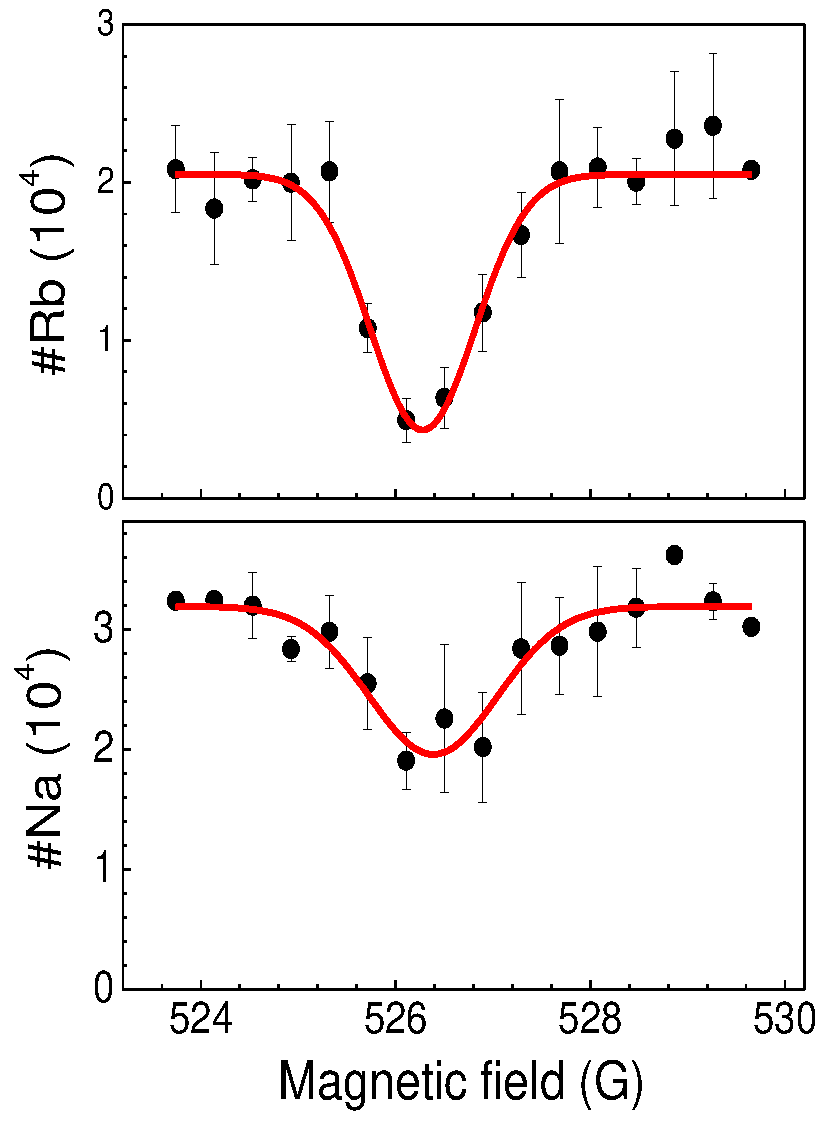
\includegraphics[width = 0.5\linewidth]{FR_loss.pdf}
\end{center}
\caption[One example of loss spectrum of Feshbach resonance.]{shows the loss spectrum of one Feshbach resonance of Na$\ket{F=1,m_F=0}$ and Rb$\ket{F=1,m_F=0}$.}
\label{FR_loss}
\end{figure}

% Introduce the dissociating method (done 2021年8月19日14:16:11)
Thus, in this Chapter, we use the most accurate method, i.e. the dissociating method, to calibrate the FR of Na and Rb at 347.64 G. To obtain an accurate map of scattering length, we need the knowledge of the molecular bound state. Recalling the discussion in chap. \ref{Chap:theory}, when we talk about quantum scattering, we typically use a pseudopotential to substitute the real complex interaction potential. However, we have to go back to the complicated real potential to obtain its scattering properties before having the scattering length. Then, an accurate map of the molecule potential is essential. Historically, people use the hot molecule to get the spectrum and then inversely deduct the potential curve \cite{}. However, this spectrum is typical only for deeply bound molecule states, which contains little information about the weakly bound states and thus the Feshbach resonances. However, our experiments need the scattering length near a Feshbach resonance, related to shallow bound states near or approaching zero when the external magnetic field is tuned across specific values. Thus, similar to the associating method, our goal is clear that we need a method to obtain these bound states energy accurately. However, to avoid the systematic error in the associating method (as shown in Fig. \ref{FR_asso}), we first form a pure molecule sample and then dissociate. Thinking in the coordinate of one molecule, one would find that this dissociation process can avoid thermal effects and thus improve the measurement accuracy. After obtaining the information of bound states, we can fit them by the coupled-channel calculation to get the Na-Rb potential. Finally, we achieve the accurate scattering length map as a function of the magnetic field. 

% Show a figure of association spectrum (done 2021年8月19日15:54:40)
\begin{figure}[htb]
\begin{center}
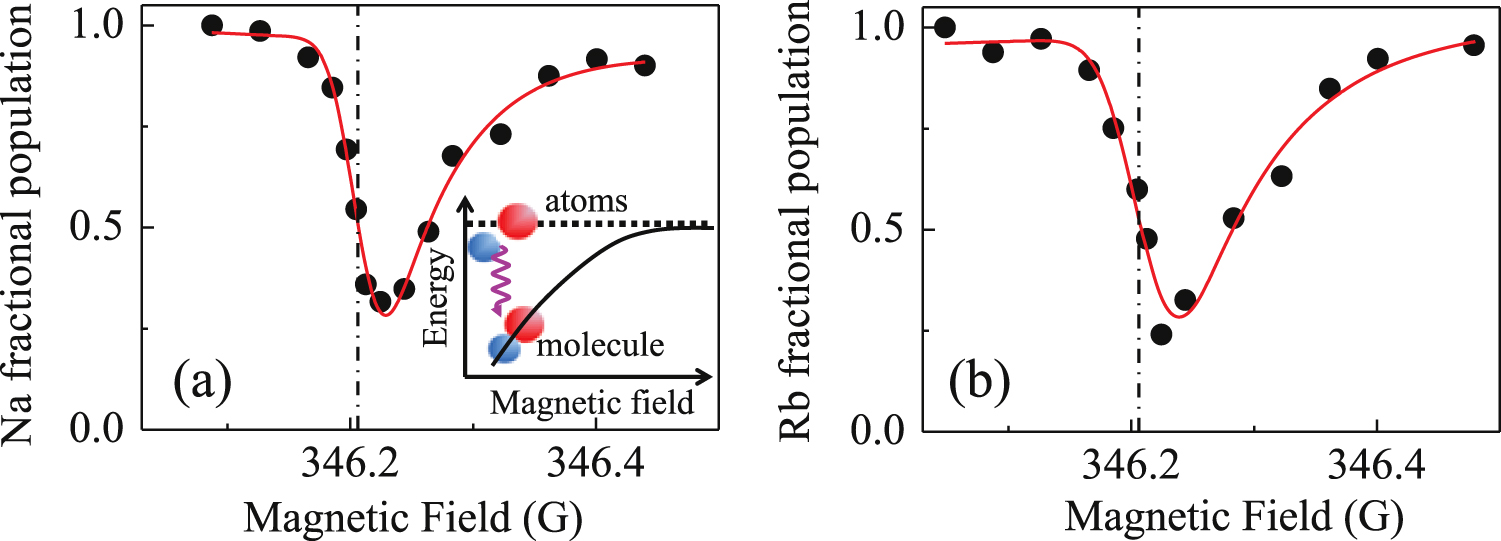
\includegraphics[width = 0.9\linewidth]{FR_asso.jpg}
\end{center}
\caption[Association spectrum of Na and Rb near 347.64 G. (Image from \cite{wang2015formation})]{Image from \cite{wang2015formation}. (a) and (b) shows the Na and Rb residue signal when doing the associating of Feshbach molecules. The dash-dot line shows the association limit, which corresponding to the zero-energy of the bound state. For a magnetic field less than the threshold, there are still association signals indicating the thermal effect. These thermal shifting and broadening smoothen the kink at the associating limit.}
\label{FR_asso}
\end{figure}

% arrangement of this chapter (done 2021年8月19日16:08:42)
The rest of this chapter is arranged as follows: Sec. \ref{sec:cali_FR} describes the method of dissociation measurement of FR molecule binding energy. Then, we apply the coupled-channel (c.c.) calculation fitting the data to obtain an accurate molecule potential curve. Finally, we achieve an accurate scattering length map. In Sec. \ref{sec:FR_spec_more}, we present ten more Feshbach resonance loss spectrums with different spin configurations of Na and Rb. They are compared to a c.c. calculation. We measured most elastic resonances and some of the inelastic, which process imaginary part of scattering length. This information can be used as a map for further exploration of a variety of Bose mixtures. Moreover, in the second part of Sec. \ref{sec:FR_spec_more} we demonstrate c.c. calculations for Rb-Rb and Na-Na both in $\ket{F=1,m_F=1}$ states. We find that the Na intraspecies interaction shows a very smooth variation from 54.5 $a_0$ (at 0 Gauss) to 64 $a_0$ (at around 900 G). This renders our estimation of Na-Na intraspecies scattering length shift about $10\%$ in the droplet paper \cite{guo2021leehuangyang}, from 54.45 $a_0$ to 60.05 $a_0$.

\section{Na-Rb Feshbach resonance at 347.64 G}
\label{sec:cali_FR}

% introduce method
This work reports new measurements of binding energies for the state that causes the FR near 347.64 G.
To reach the highest accuracy, we implement the dissociation method to measure the binding energies. We achieve magnetic field stability at the mG level. The data are used to refine the interaction potentials for the $X^1\Sigma^+$ and $a^3\Sigma^+$ electronic states by fitting to coupled-channel bound-state calculations. We then use coupled-channel scattering calculations to obtain a highly accurate mapping $a(B)$ for the FR near 347.64~G. This has become a cornerstone for our recent experiment on the heteronuclear \Na--\Rb quantum droplet. We also report 10 $s$-wave FRs in different combinations of Zeeman levels $m_F$ in the atomic $F = 1$ manifolds, measured by the inelastic loss method. These new resonances may find applications in future explorations of the \Na--\Rb system.
Currently, the most accurate method of characterizing a FR relies on measurements of the binding energy $E_{\rm b}$ of FMs by dissociation~\cite{Bartenstein2005,Lompe2013,Chin2005Radio,Chapurin2019}. The singlet and triplet interaction potentials between the atoms can then be determined precisely by fitting the binding energies using coupled-channel bound-state calculations. The interaction potentials can then be used to calculate the correspondence $a(B)$ between the magnetic field $B$ and the scattering length $a$ using coupled-channel scattering calculations. In simple cases, $a(B)$ can be represented by Eq.~\ref{eq1} with FR parameters $a_{\rm bg}$, $B_0$, and $\Delta$.

% method detailed
The most accurate method of characterizing a FR relies on measurements of the binding energy $E_{\rm b}$ of FMs by dissociation~\cite{Bartenstein2005,Lompe2013,Chin2005Radio,Chapurin2019}. This can be achieved by applying a radio-frequency pulse to drive a bound-free transition~\cite{Bartenstein2005,Lompe2013,Chapurin2019}. The binding energy is obtained by subtracting the free-free transition energy from the bound-free transition energy. In the current work, as shown schematically in Fig.~\ref{fig1}(a), the FM lies very close in energy to the free atom pair. In this case, the dissociation can be driven by magnetic field modulation spectroscopy~\cite{Claussen2003,Thompson2005}. As illustrated in Fig.~\ref{fig1}(b), this is implemented by adding a small-amplitude oscillation to the magnetic field after the magnetoassociation. The oscillating magnetic field can be expressed as $B + A \, {\rm sin}(2\pi f t)$, with $B$ the final magnetic field that determines $E_{\rm b}$, $A\ll B_0-B $ and $f$ the modulation amplitude and frequency, respectively. Dissociation starts to occur when $f$ matches $E_{\rm b}/h$. For $f > E_{\rm b}/h$, the excess energy is converted to kinetic energy of the free atoms as $E_{\rm k} = hf - E_{\rm b}$. Due to the variation of the bound-free Franck-Condon factor with $E_{\rm k}$~\cite{Chin2005Radio}, the dissociation spectrum is typically asymmetric and broad with respect to $f$.

\subsection{Production of pure Feshbach molecule sample}

% produce atom to molecule
Our experiment starts from an optically trapped ultracold mixture of \Na and \Rb atoms, both in their lowest hyperfine state $\ket{F = 1, m_F = 1}$~\cite{Wang2013,wang2015,Jia2020}. Magnetoassociation starts from an initial magnetic field of 350 G, just above the FR at $B_0 = 347.64$~G. The magnetic field is ramped down across the resonance to form FMs, and then to 335.6 G. At this field, the FMs have a nearly zero magnetic dipole moment; this allows us to remove the residual atoms with a short and strong magnetic field gradient without losing molecules. Afterwards, the magnetic field is ramped up to a range of target values below $B_0$ for further experiments. Following this procedure, we can routinely obtain a pure sample of \NaRb FMs with a typical temperature of 300 nK and a trap lifetime of more than 30 ms. This short lifetime is due to near-resonance photon scattering by the 947 nm optical trap light~\cite{Guo2017,Jia2020}, which is provided by a home-built diode laser system. In another experiment on \NaRb, in which a single-frequency 1064 nm laser is used as the optical trap light, FM lifetimes greater than 100 ms have been observed~\cite{Wang2019,guo2021}. Nevertheless, the current lifetime is more than enough for the present work, as we need only 10 ms for magnetic field stabilization and less than 1 ms for dissociation.
Our experiment starts from an optically trapped ultracold mixture of \Na and \Rb atom both in their lowest hyperfine state $\ket{F = 1, m_F = 1}$. The magnetoassociation of FMs via the $B_0 = 347.64$~G FR starts from an initial magnetic field at 350 G. The magnetic field is then ramped down crossing the resonance and then to 335.6 G. At this field, the FMs have a nearly zero magnetic dipole moment which allows us to remove the residual atoms with a short and strong magnetic field gradient without causing loss of FMs. Afterwards, the magnetic field is ramped up to a range of target values below $B_0$ for further experiments. Following this procedure, we can routinely obtain a pure sample of \NaRb FMs with a typical temperature of 300 nK and a trap lifetime of more than 20 ms. This short lifetime is most probably due to accidental near resonance photon scattering by the \textcolor{blue}{947 nm} optical trap light which has a specified linewidth of 3 nm. In the ground-state \NaRb experiment, which is using a single frequency 1064 nm laser as the optical trap light, a FM lifetime more than 100 ms has been observed. Nevertheless, the current lifetime is more than enough for this work as we only need 10 ms for the magnetic field stabilization and less than 1 ms for the dissociation.  

% How to remove residue atom as fast as possible
To remove residue atom from molecule sample, we need to identify them by different properties of them, such as their magnetic dipole, mass, transition energy and so on. To blast atom away, we need achieve as large as possible accelaration for atom, which requires as strong field as possible. Typical method can be magnetic gradient, species dependent optical dipole force (tune-in, tune-out trap) and resonance light. The largest way is using the resonance light which can generate a accelaration about 10000 m/s2 for typical alkali atom. For our case, the Na and Rb are both in F=1 and mF=1 state, which can be driven by a sigma- light to F'=0 state (check). This is a quasi-cycling transition which possess a reloading rate about \(90\%\). The leackage part can be pumped to other dark states, thus this transation can be used directly. So, we typical first transfer atom to F=2 and mF=2 state by light or by MW, than using the image cycling transition to remove the atom clearly. %我们用过1,1的pump光做过吗?check
With the newly upgrade full-wave loop antenna, we can achieve a high Rabi freq for both Na and Rb up to 50kHz. Then, a 10 us pulse could transfer all atom to the cycling transition ground state F=2, mF=2.  

\subsection{Dissociation method for measuring binding energy of Feshbach molecule}


\begin{figure}[hb]
\begin{center}
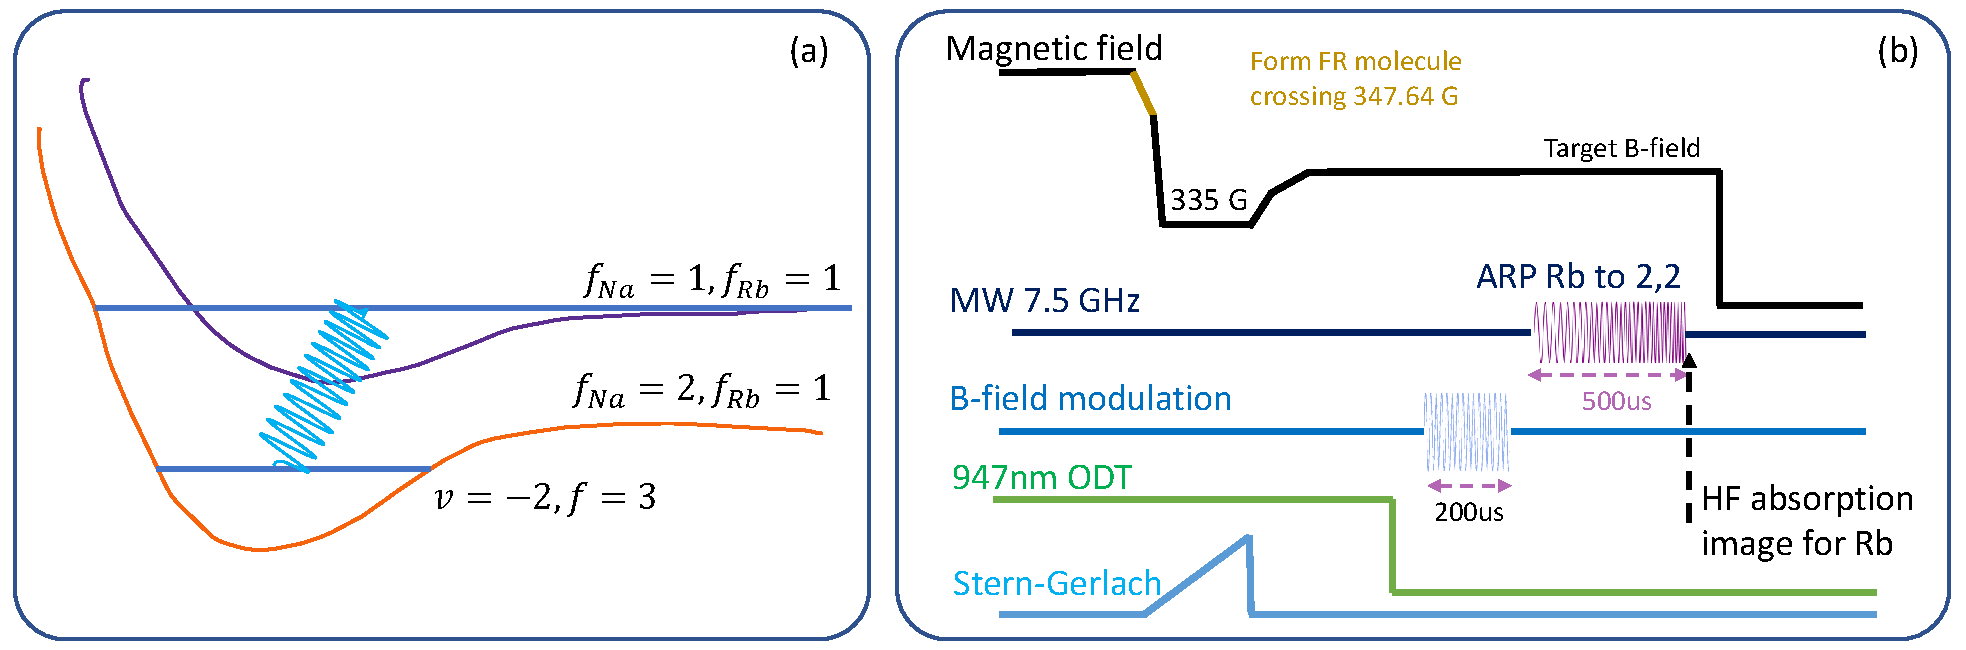
\includegraphics[width = 0.9\linewidth]{FR_dis.pdf}
\end{center}
\caption[Time sequence for measuring binding energy of Feshbach molecules]{Measuring the binding energy of a Feshbach molecule with magnetic field modulation spectroscopy. (a) The binding energy of the FM is $E_{\rm b}$. A bound-free transition can be driven by an oscillating magnetic field. (b) The FMs are first created by ramping the magnetic field across $B_0$. After the magnetic field is stabilized to its final value, a small-amplitude sinusoidal oscillation at frequency $f$ near $E_{\rm b}/h$ is added to dissociate the FMs and measure the binding energy. See the text for a more detailed description of the magnetic field ramping procedure.}
\label{FR_dis}
\end{figure}


% magnetic field modulation method
The magnetic field modulation is generated by a single loop coil driven by a low frequency high power radio frequency amplifier. The single loop coil is placed just above the vacuum cell and coaxially with the Feshbach coils so that an $Am$ of several mG can be added to the large magnetic field. The coil has a limited modulation bandwidth of about 2 MHz. To avoid the ac Stark shift from the trapping light, the optical trap was turned off 50 $\mu s$ before applying the magnetic field modulation pulse. This will also reduce possible systematic errors induced by mean-field shifts of both the FMs and the free atoms as the density of FMs is lowered. The magnetic field modulation pulse duration is chosen empirically so that the fraction of dissociation is no more than \textcolor{blue}{70 \%}. This is a compromise for detection signal-to-noise ratio and the requirement for using the Fermi Golden rule to fit the dissociation lineshape which is only strictly followed for weak coupling. 

% dissociation signal
The dissociation signal is detected by absorption imaging of the fragmented \Rb atoms. Fig.~\ref{fig2}(a) and (b) show two example dissociation spectra versus the modulation frequency $f$ for FMs at 347.371(5) G and 346.000(5) G, respectively. Here the magnetic field is measured with radio frequency spectroscopy of the Rb atoms. Threshold behaviors are clearly visible in both dissociation spectra. For Fig.~\ref{fig2}(a), no dissociation is observed for $f$ below 60 kHz; while in Fig.~\ref{fig2}(b), the threshold is near 1.3 MHz. Since the dissociation process involves no moment transfer, the dissociation threshold is an accurate measurement of the binding energy $E_b$ of the FM. Above this threshold, the profile of the spectrum is determined by the overlap between the wave functions of the bound and free states. As the excessive energy $hf-E_b$ will be converted into the relative motion of the two atoms, the wave function of the free atoms and thus the bound-free transition rate changes with $f$. Following~\cite{Mohapatra2015}, the lineshape of magnetic field modulation spectroscopy can be represented as 
\begin{equation}
N_{Rb}(f) \propto \frac{\sqrt{hf-E_b}}{hf}.
\label{eq2}
\end{equation}
From this lineshape, a dissociation maximum should be observed at $f = 2E_b/h$, afterwards, the signal will decay with a long tail following $1/\sqrt{f}$. The spectrum in Fig.~\ref{fig2}(a) follows this lineshape well. For the spectrum in Fig.~\ref{fig2}(b), the maximum is not reached due to the limited modulation bandwidth. The same is true for all the spectra with $E_b>1$~MHz.   

%%% dissociation curve %%%
\begin{figure}[t]
\begin{center}
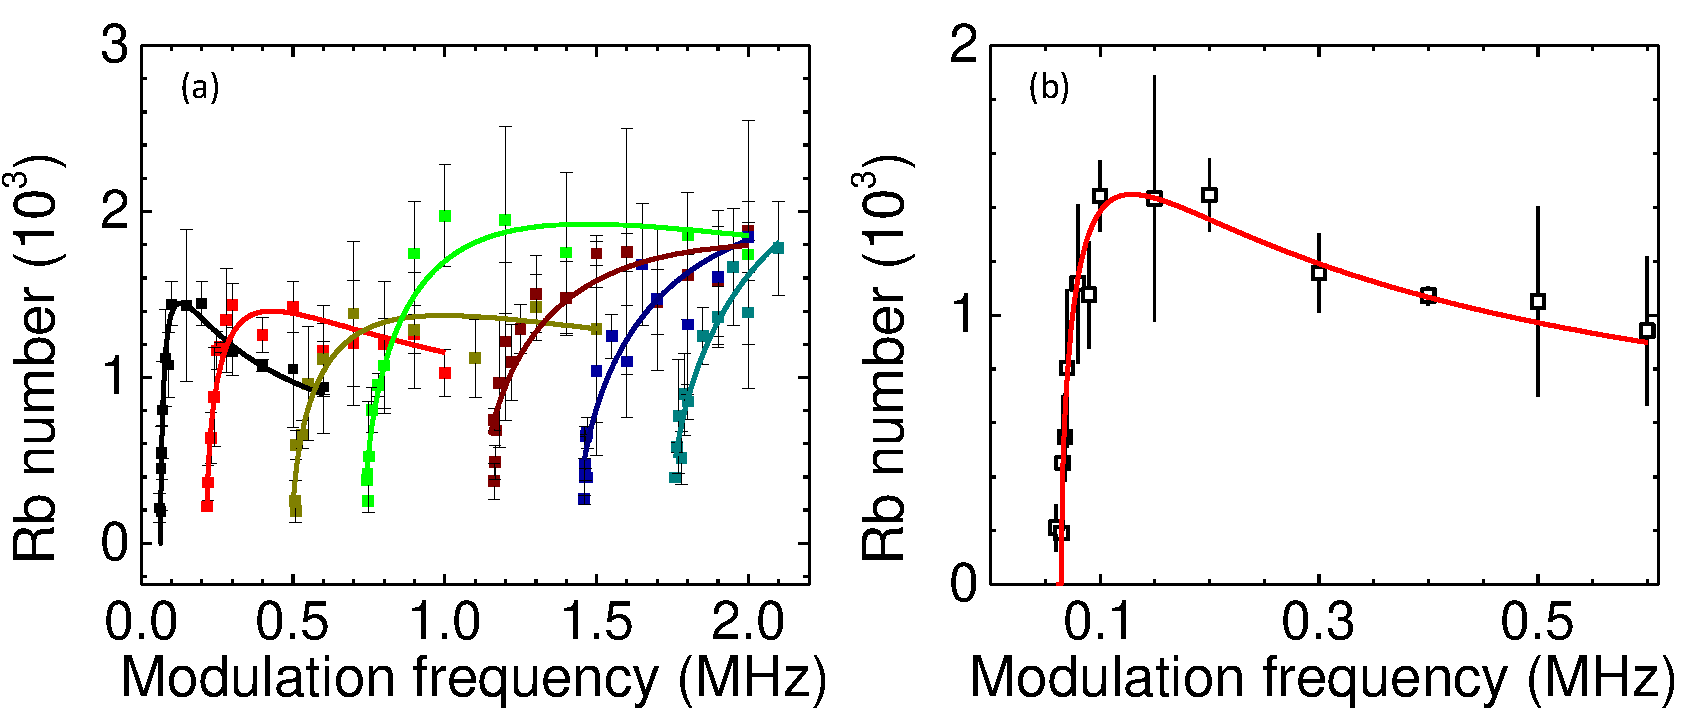
\includegraphics[width = 0.95\linewidth]{FR_spec.pdf}
\end{center}
\caption[Feshbach molecule dissociation spectrum]{Feshbach molecule dissociation spectrum at magnetic field of (a) 347.371 G, and (b) 346.000 G. The red solid curves are fitted to Eq.~\ref{eq2} to extract the FM binding energies. Because of the limited modulation bandwidth of the single-loop coil, only part of the spectrum is accessible in (b).}
\label{FR_spec}
\end{figure}
%%% dissociation curve %%%



To determine the dissociation threshold, we fit each spectrum with Eq.~\ref{eq2}. For partial dissociation spectra like Fig.~\ref{fig2}(b), we have verified with simulated data that $E_{\rm b}$ can still be determined with uncertainties less than 5 kHz. The variation of $E_{\rm b}$ with magnetic field, over a range from 0.061 MHz to 1.739 MHz, is plotted in Fig.~\ref{fig3}(a) as blue open circles. The error bar for each $E_{\rm b}$ is smaller than the symbol size. The uncertainty in the measured magnetic field is $\pm3$~mG. 

%%% Binding energy vs. Magnetic field %%%
\begin{figure}[htbp]
\begin{center}
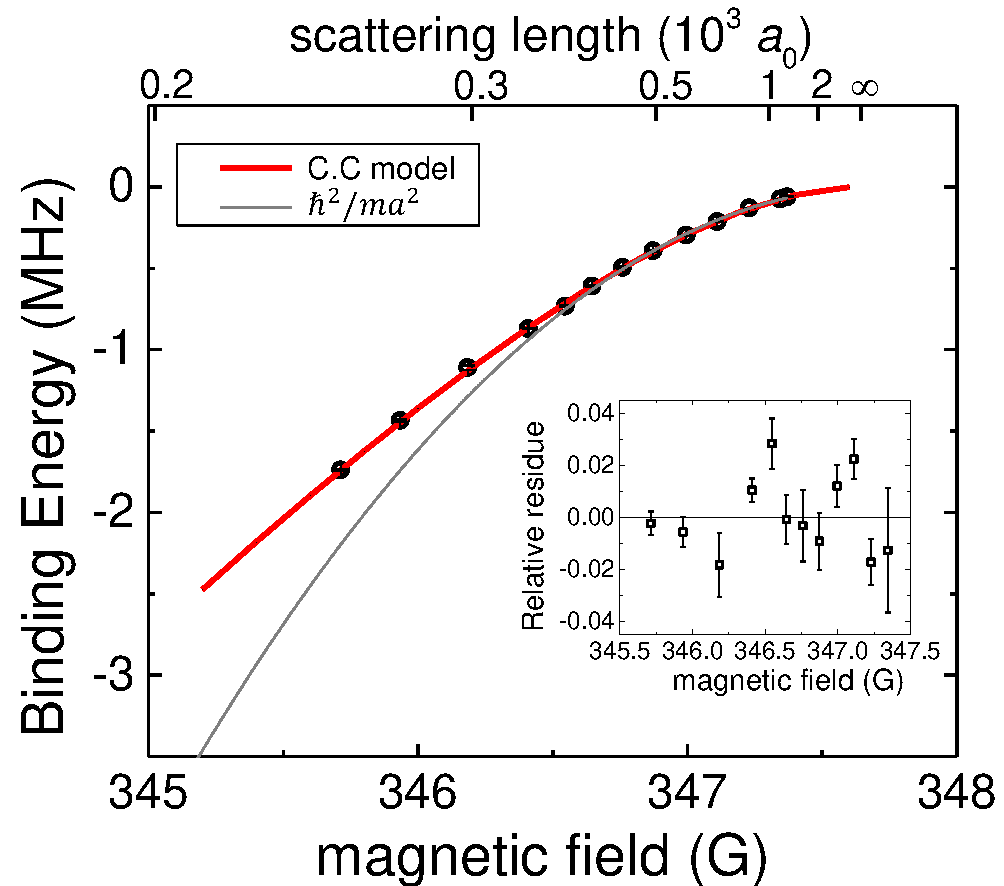
\includegraphics[width = 0.9\linewidth]{FR_bind.pdf}
\end{center}
\caption[Binding energy of \NaRb~Feshbach molecules at 347.64 G]{(a) Binding energy of \NaRb~Feshbach molecules created via the FR near 347.64 G in the entrance channel Na$\ket{1,1}+$Rb$\ket{1,1}$. The blue open circles are the data points measured in this work with the dissociation method. The error bars are smaller than the symbol size. The red solid curve is from the coupled-channel fitting, while the black dashed curve is from the universal model. (b) and (c) show the comparison between the previously observed binding energies~\cite{wang2015} (black open squares), measured using the association method, and the calculations (red solid curves) from the present coupled-channel model, for FMs created near the FRs at 347.64 G and 478.7 G, respectively.}
\label{FR_bind}
\end{figure}
%%% Binding energy vs. Magnetic field %%%

Figure~\ref{fig3} (b) and (c) show $E_{\rm b}$ for FMs that were obtained in 2015 with the association method~\cite{wang2015} near the resonances at 347.64 G and 478.7 G. In that work~\cite{wang2015}, the binding energy was fitted using the square-well model~\cite{Lange2009} with a fixed background scattering length $a_{\rm bg} = 66.77a_0$. This value of $a_{\rm bg}$ was obtained from the coupled-channel modeling of the several Feshbach resonances observed with atom-loss spectroscopy in 2013~\cite{Wang2013}. However, the square-well model requires $a_{\rm bg}$ much larger than the interaction range, which is set by the mean scattering length of the van der Waals potential \cite{Gribakin1993}; this is $\bar{a} = 55.2\,a_0$ for \NaRb. This condition is not satisfied for the Feshbach resonances considered here. It is also well known that resonance positions measured by atom-loss spectroscopy are not accurate enough, due to the complicated dynamics of three-body recombination. These issues all contribute to the inaccuracy of the Feshbach resonance parameters determined previously~\cite{wang2015}. In the following, we solve these issues with a new coupled-channel modeling of the binding energies of the FMs.

\subsection{Coupled-channel modeling and FR parameters}
% Why talk about CC

After obtaining the binding energy of Feshbach molecule, we actually measure out how the highest shallow bound state energy varying with magnetic field. This very shallow bound sate actually affected by the shortest part and the long range part (C6,C8,C10) of the molecular potential curve. So, by the above measurement, we can calibrate the potential more precisely, especially at short and long range. Since a typical molecular potential is achieved by "FRTS" (check name), which mainly use the information for the deep binding bound state, i.e. middle range  potential. As shown in the Figure(add). 

\begin{figure}[htbp]
\begin{center}
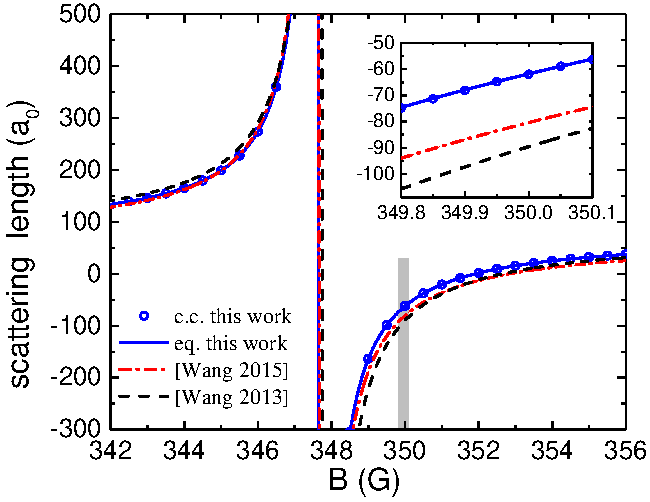
\includegraphics[width = 0.9\linewidth]{FR_para.pdf}
\end{center}
\caption[Scattering length as function of magnetic field]{Comparison of the mapping between magnetic field and scattering length with Feshbach resonance parameters obtained in this work, using coupled-channel results directly (blue open circles) and fitted to Eq.~\ref{eq1} (blue solid curve) and , and in Ref.~\cite{wang2015} (red dash-dotted curve) and Ref.~\cite{Wang2013} (black dashed curve), both using Eq.~\ref{eq:FRsum}. The region of interest for the droplet experiment~\cite{guo2021}, marked with a vertical gray bar, is enlarged in the inset. }
\label{FR_para}
\end{figure}
%%% Binding energy vs. Magnetic field %%%


\section{Na-Rb, Na-Na and Rb-Rb scattering length summery}
\label{sec:FR_spec_more}
% overview
Besides the Feshbach resonance at 347.64 G, different combinations of spin state of Na and Rb possess plenty of FRs. Ref.~\cite{Wang2013} investigated the entrance channels $\ket{1}+\ket{1}$ and $\ket{-1}+\ket{-1}$ and in total observed three $s$-wave and two $p$-wave FRs. In addition, ten more $s$-wave FRs were predicted for collisions between pairs of atoms in different $F = 1$ hyperfine Zeeman states. In this section, we report the experimental observation of several of these FRs below 1000 G in 5 hyperfine Zeeman combinations. We believe these FRs will find important applications in the future, for example in the investigation of BEC mixtures and quantum droplets with more than two components~\cite{ma2021}. 

% some words on the Na-Na scattering length
With the powerful tool MOLSCAT, we can get more precise map of scattering length and magnetic field. Since even the background scattering length varies when external field changing, the value of the scattering length especially for finite (not low) field should be paid more attention to. Here we find that the Na-Na 1,1 state have a smoothly varying background scattering length from low field to around 900 G (near the FR). Its value starts from 54.45 $a_0$ to about 64 $a_0$. For our droplet experiment, under about 350 G magnetic field, the Na-Na scattering length actually is 60.05 $a_0$ which larger about 10\% then it at low field.

\subsection{Na-Rb scattering length for different spin combination}

For simplicity, we will denote the collision channel of a pair of \Na + \Rb atoms by $\ket{m_F^{\rm Na}}+\ket{m_F^{\rm Rb}}$. In ref.~\cite{Wang2013}, both the $\ket{1}+\ket{1}$ and the $\ket{-1}+\ket{-1}$ channels were investigated and in total 3 $s$-wave and 2 $p$-wave FRs were observed. As shown in Figreu(add), we detect more FRs in different combinations. The experiment for this section starts from optically trapped thermal mixtures of \Na and \Rb both in the $\ket{-1}+\ket{-1}$ channel. The number of atoms for both species are typically around $10^5$ and the sample temperatures are about 1~$\mu$K. The atoms are then transferred to selected hyperfine Zeeman levels with radio frequency (rf) rapid adiabatic passages. For each species, the $\ket{-1}\rightarrow \ket{0}$ and the $\ket{0}\rightarrow \ket{1}$ Zeeman splittings are very similar. In addition, these splittings in different species are also very similar to each other. To avoid cascade transitions and to realize species-selective state control, the state transfers are performed at \textcolor{blue}{100 G} where the transitions are all different by more than 500 kHz. With this method, we are able to prepare the Na-Rb mixture in all the 9 possible $m_F$ combinations of their $F = 1$ states. 
After the state preparation, we ramp the magnetic field to different values and hold the samples for 50 ms \textcolor{blue}{not all data points are holding 50 ms, the loss width may be related to holding duration} before releasing the atoms from the optical trap and measuring the remained numbers of atoms. Intersperses FRs manifest as losses of atoms in both \Na and \Rb atoms as a result of enhanced interspecies three-body recombination rates. As presented in Fig.~\ref{fig4}, guided by the predictions in~\cite{Wang2013}, we observe 10 FRs in 6 hyperfine Zeeman combinations. 

%%% add figure of FR spectroscopy %%%
\begin{figure}[htb]
\begin{center}
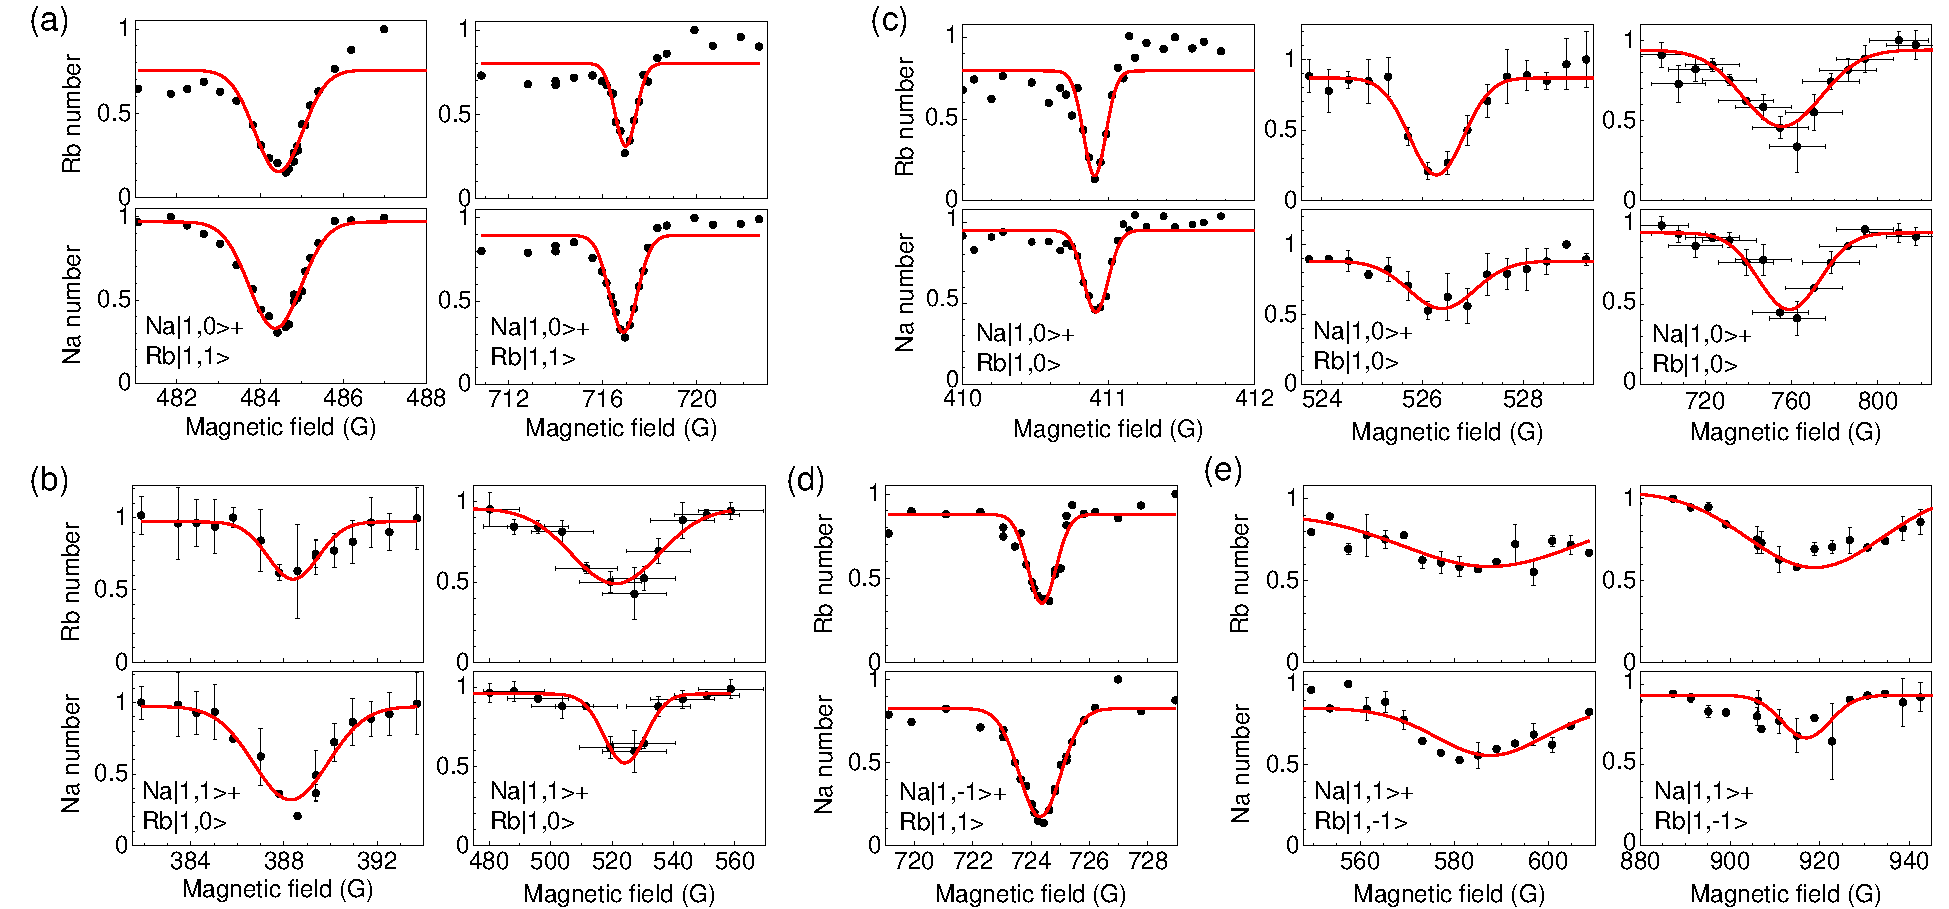
\includegraphics[width = \linewidth]{FR_more.pdf}
\end{center}
\caption[Loss spectroscopy of Feshbach resonance with different spin combinations]{Feshbach resonances in \Na-\Rb, observed by losses for atoms in the $F = 1$ hyperfine states. (a) and (b) are for the two channels in the $M_F = 1$ manifold; (c), (d) and (e) are for the three channels in the $M_F = 0$ manifold. The typical holding time at each magnetic field is 50 ms. The solid curves are from Gaussian fitting to determine the lineshape center. Error bars for the atom numbers represent one standard deviation. The large error bars for the magnetic field for the several broad loss spectra are due to less precise magnetic field control in these cases (see text).}
\label{FR_more}
\end{figure}

\begin{figure}[tb]
\begin{center}
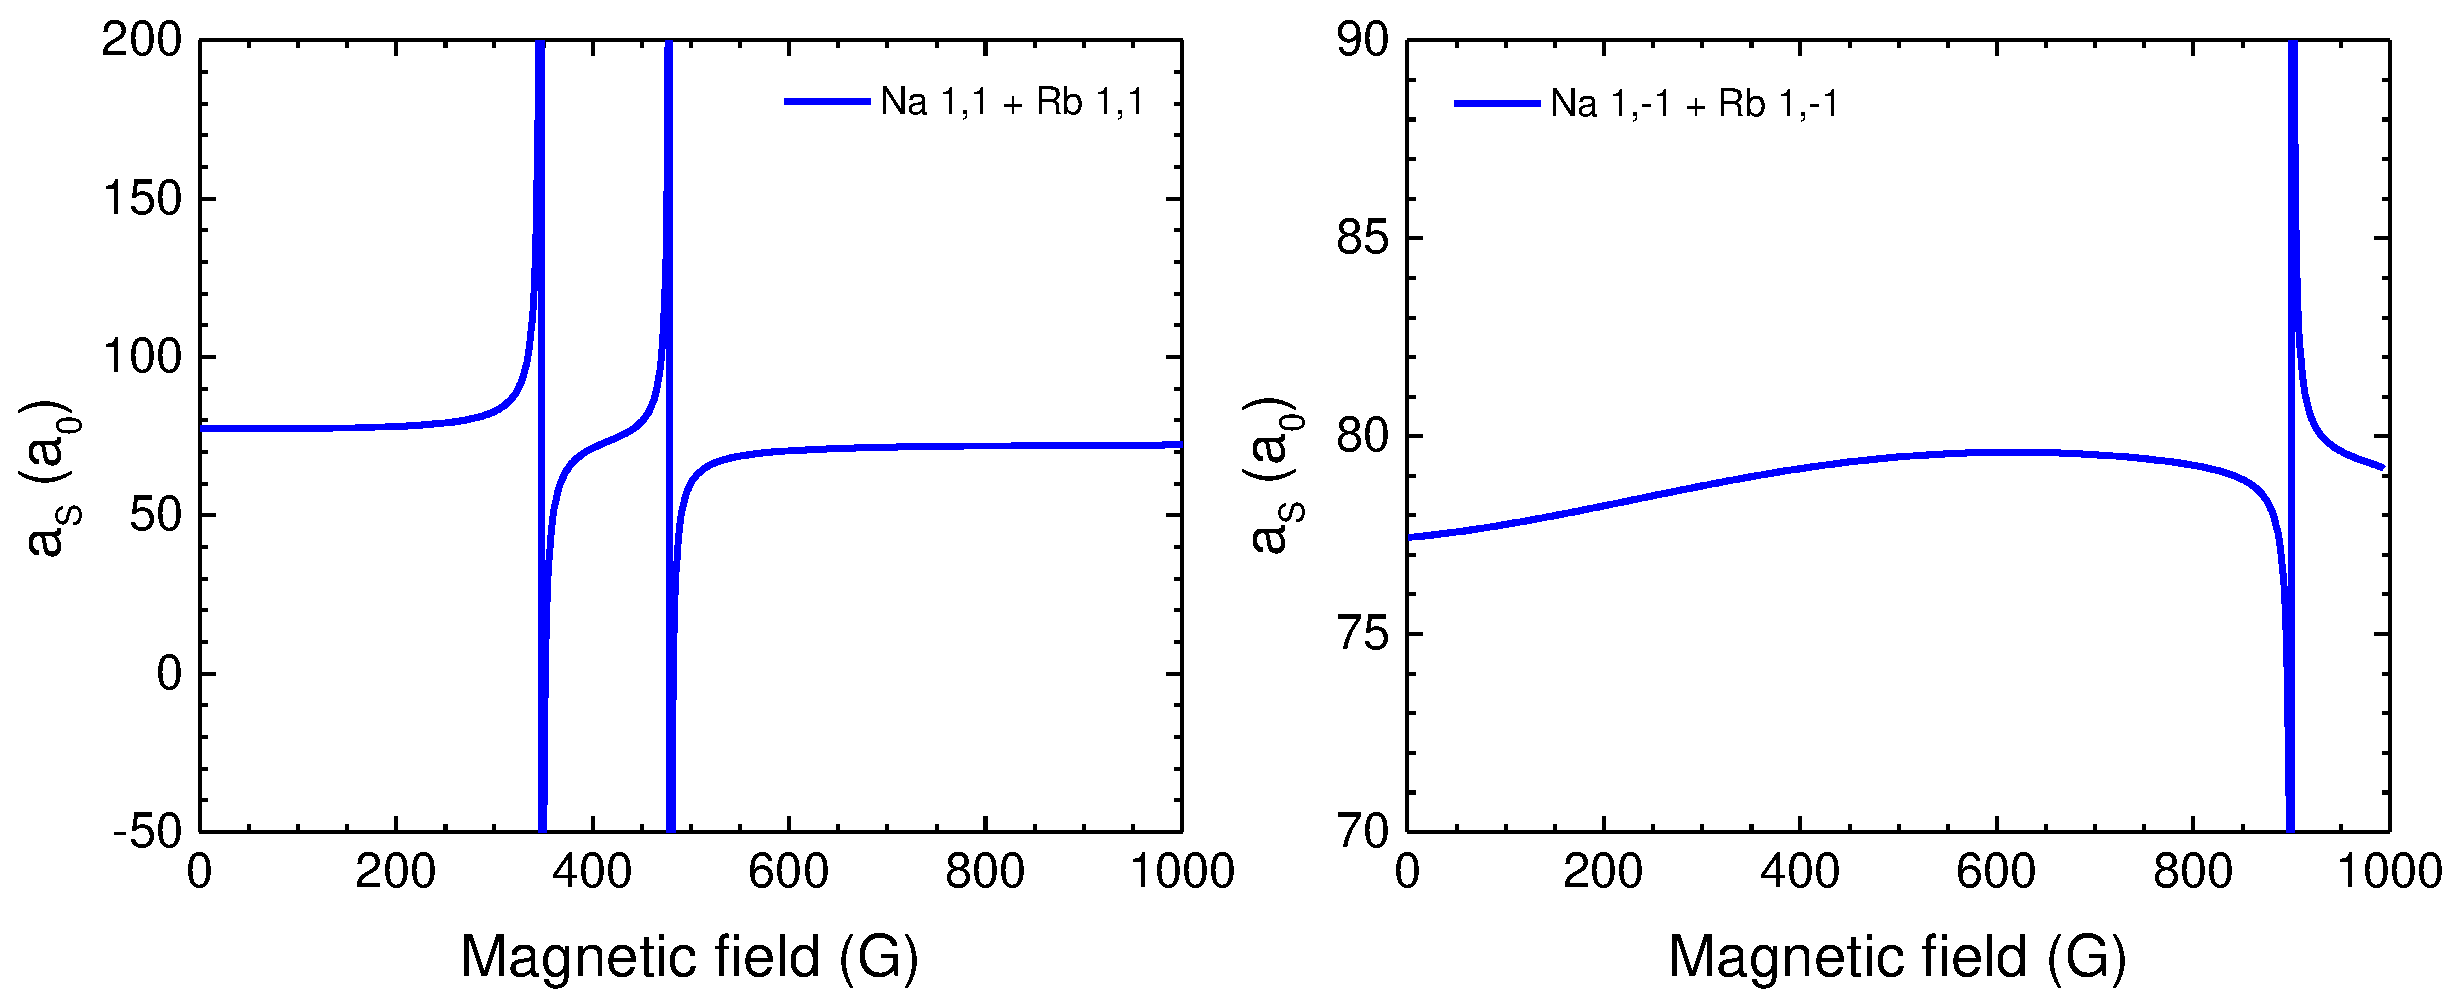
\includegraphics[width = \linewidth]{FR_groupAE.pdf}
\end{center}
\caption{}
\label{FR_groupAE}
\end{figure}

\begin{figure}[tb]
\begin{center}
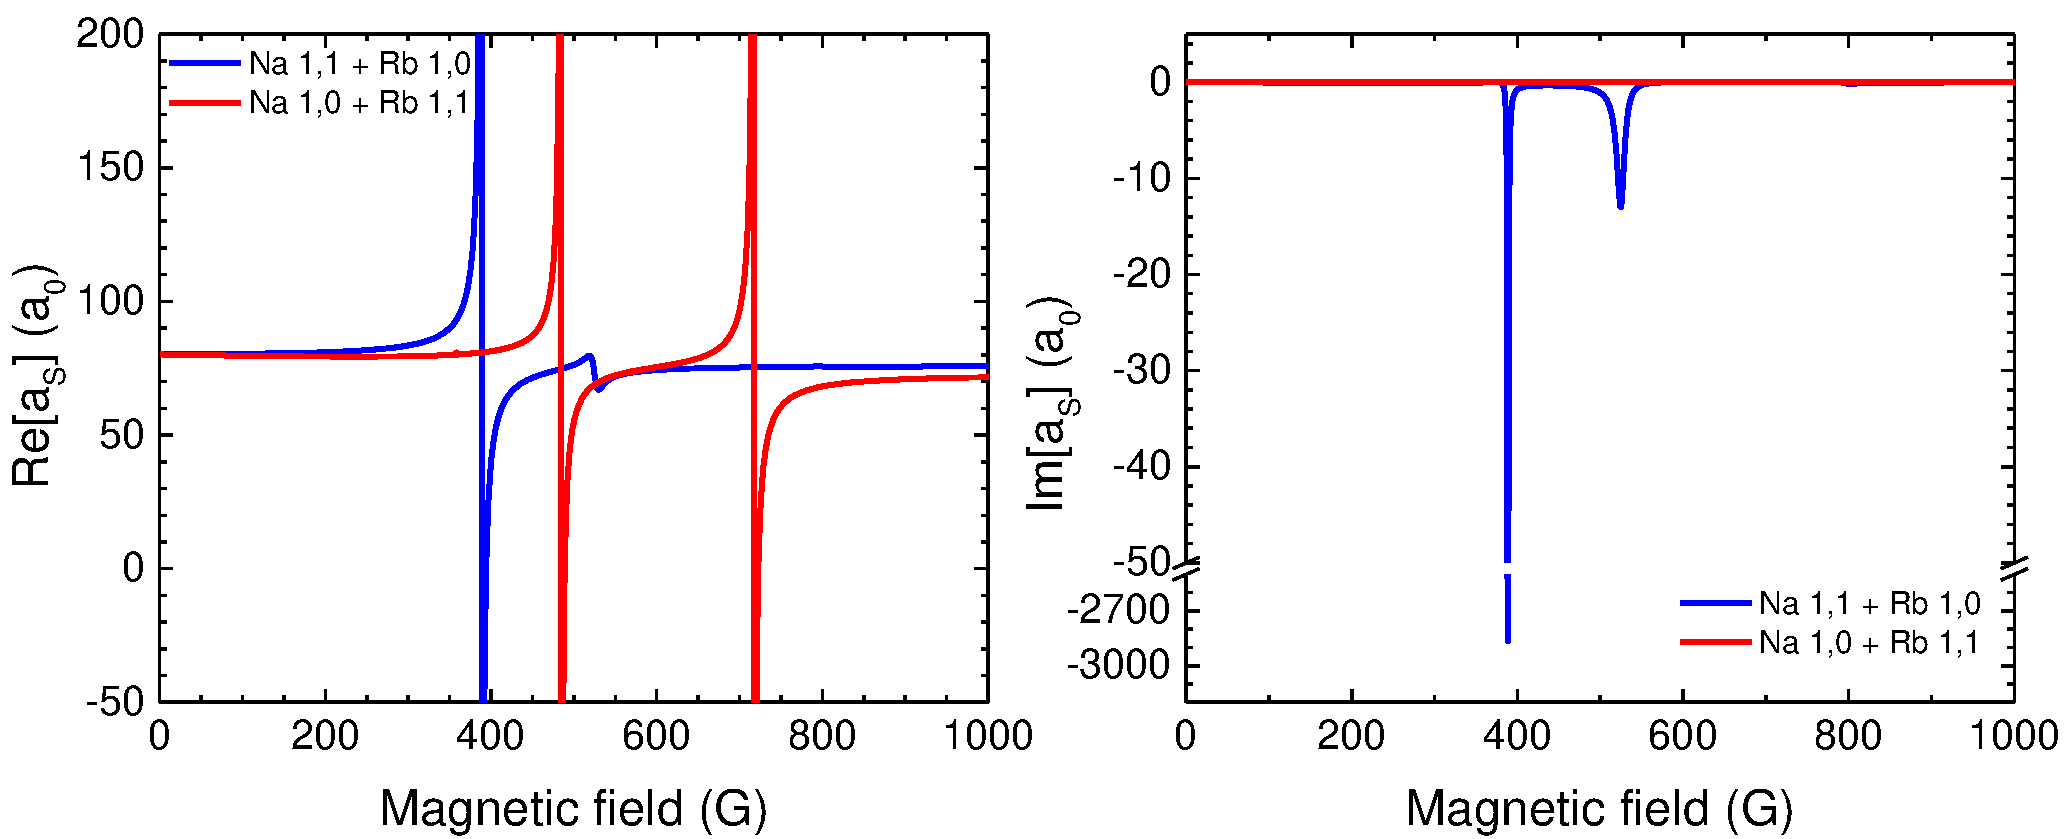
\includegraphics[width = \linewidth]{FR_groupB.pdf}
\end{center}
\caption{}
\label{FR_groupB}
\end{figure}

\begin{figure}[tb]
\begin{center}
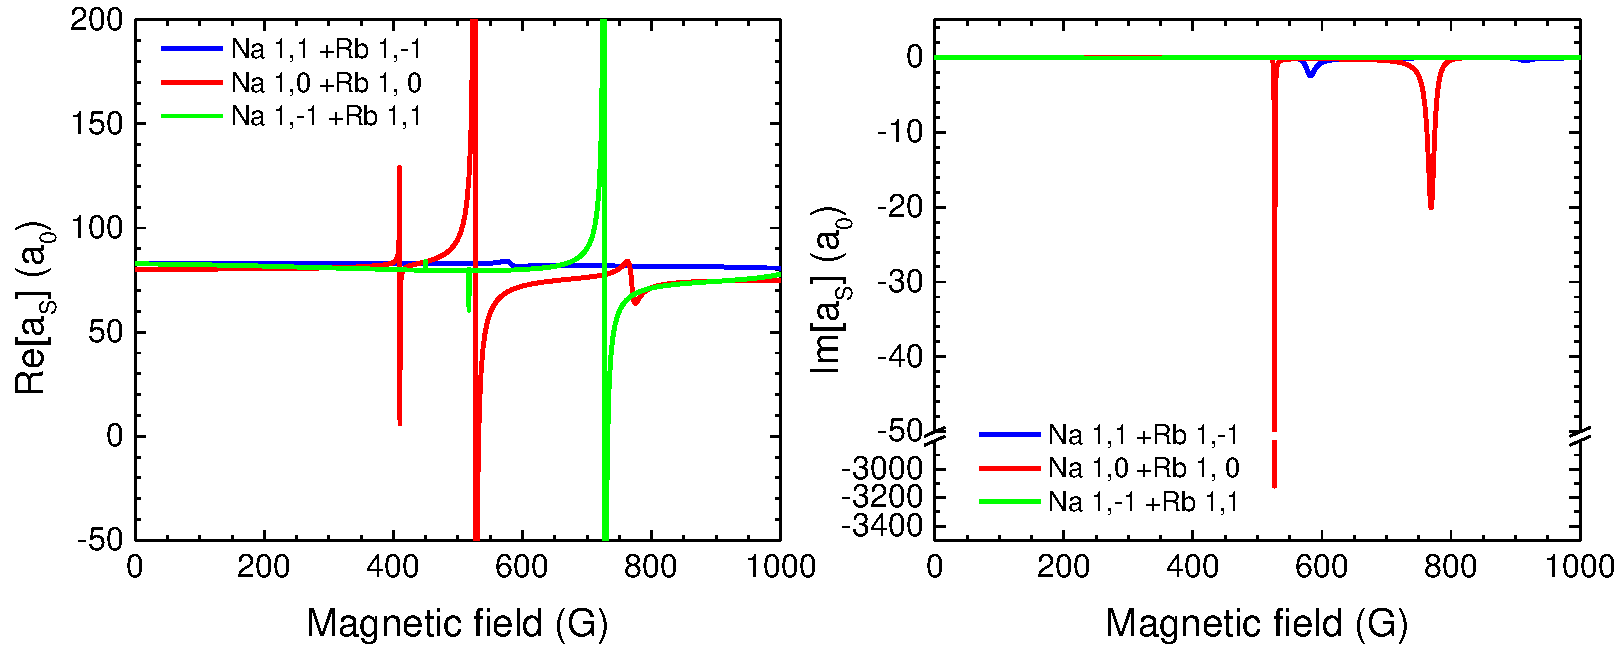
\includegraphics[width = \linewidth]{FR_groupC.pdf}
\end{center}
\caption{}
\label{FR_groupC}
\end{figure}

\begin{figure}[tb]
\begin{center}
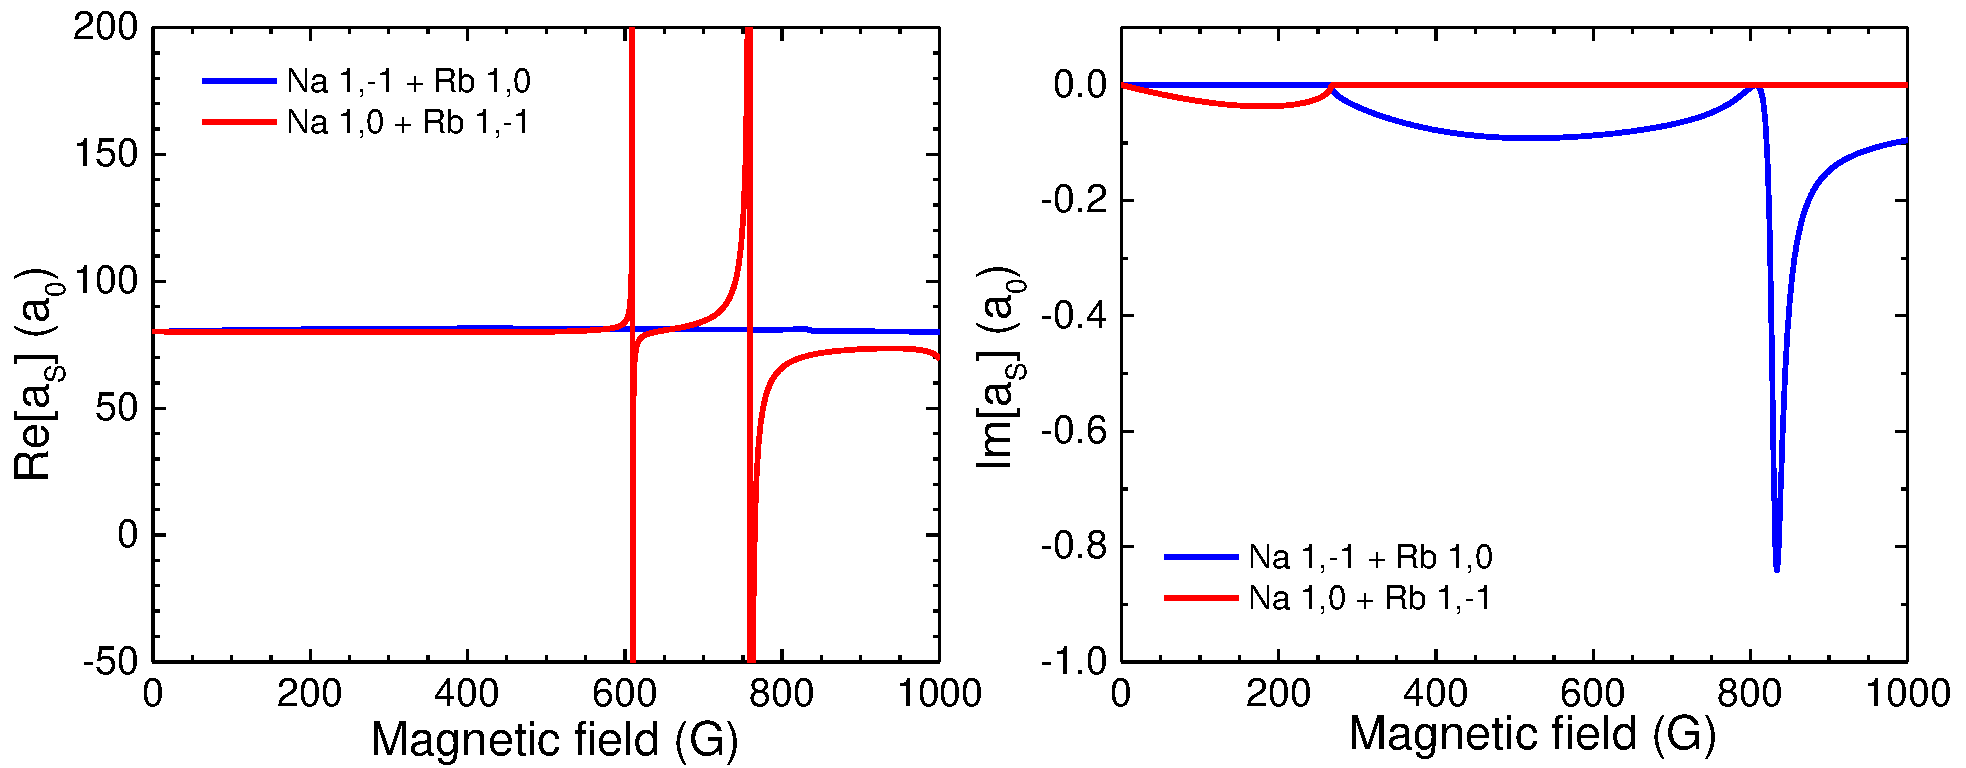
\includegraphics[width = \linewidth]{FR_groupD.pdf}
\end{center}
\caption{}
\label{FR_groupD}
\end{figure}

\begin{figure}[tb]
\begin{center}
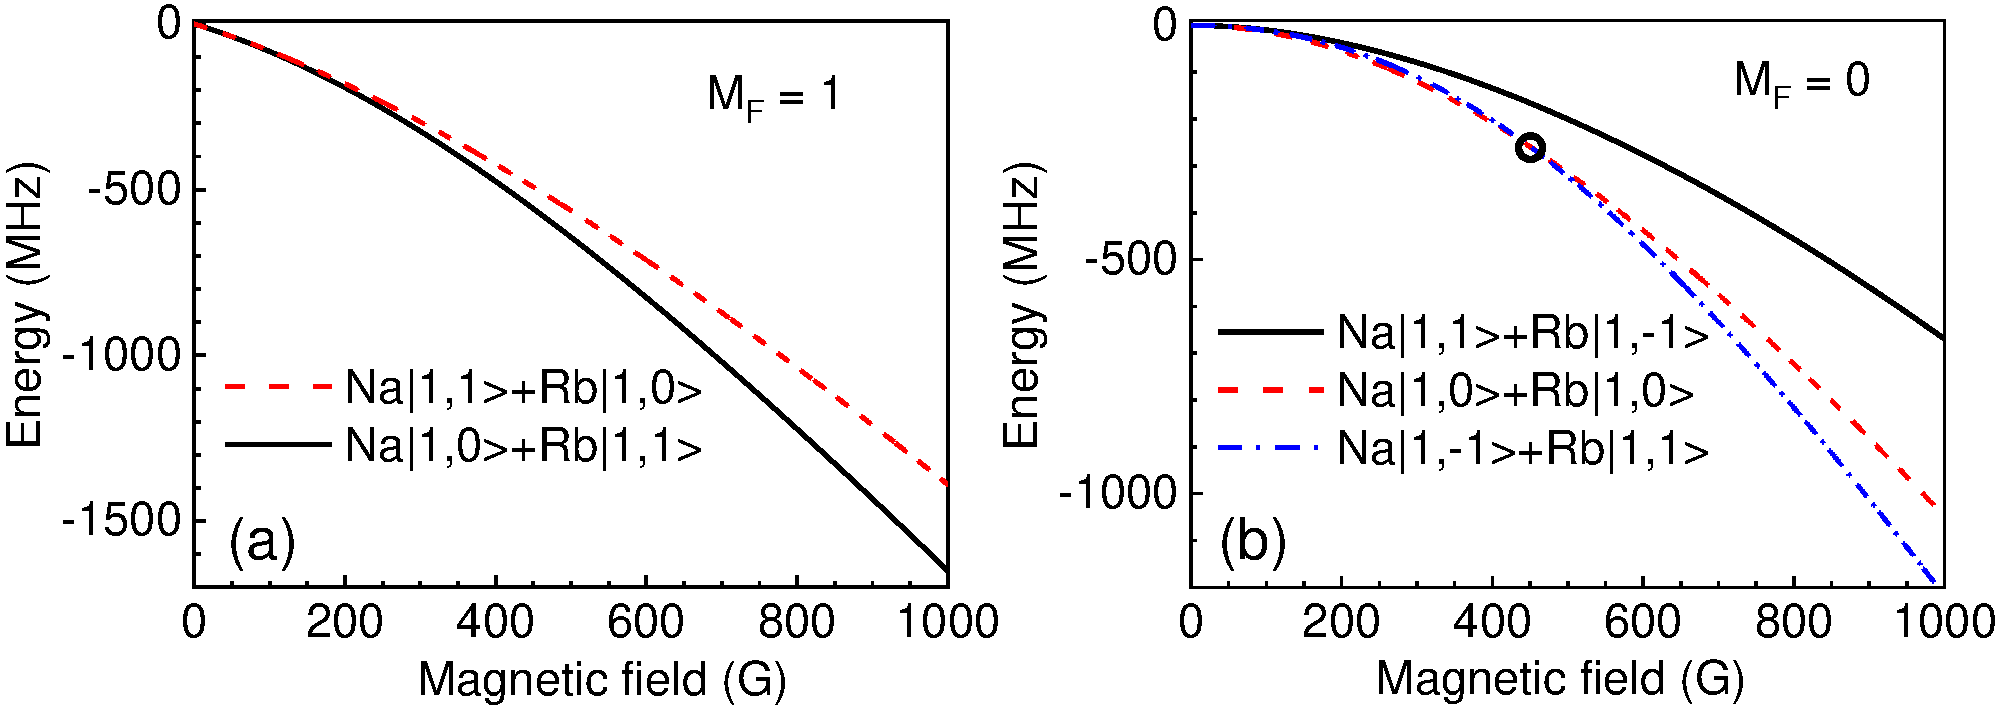
\includegraphics[width = \linewidth]{FR_Zeeman-BC.pdf}
\end{center}
\caption{}
\label{FR_Zeeman-BC}
\end{figure}

\subsection{Na-Na and Rb-Rb scattering length}

\begin{figure}[tb]
\begin{center}
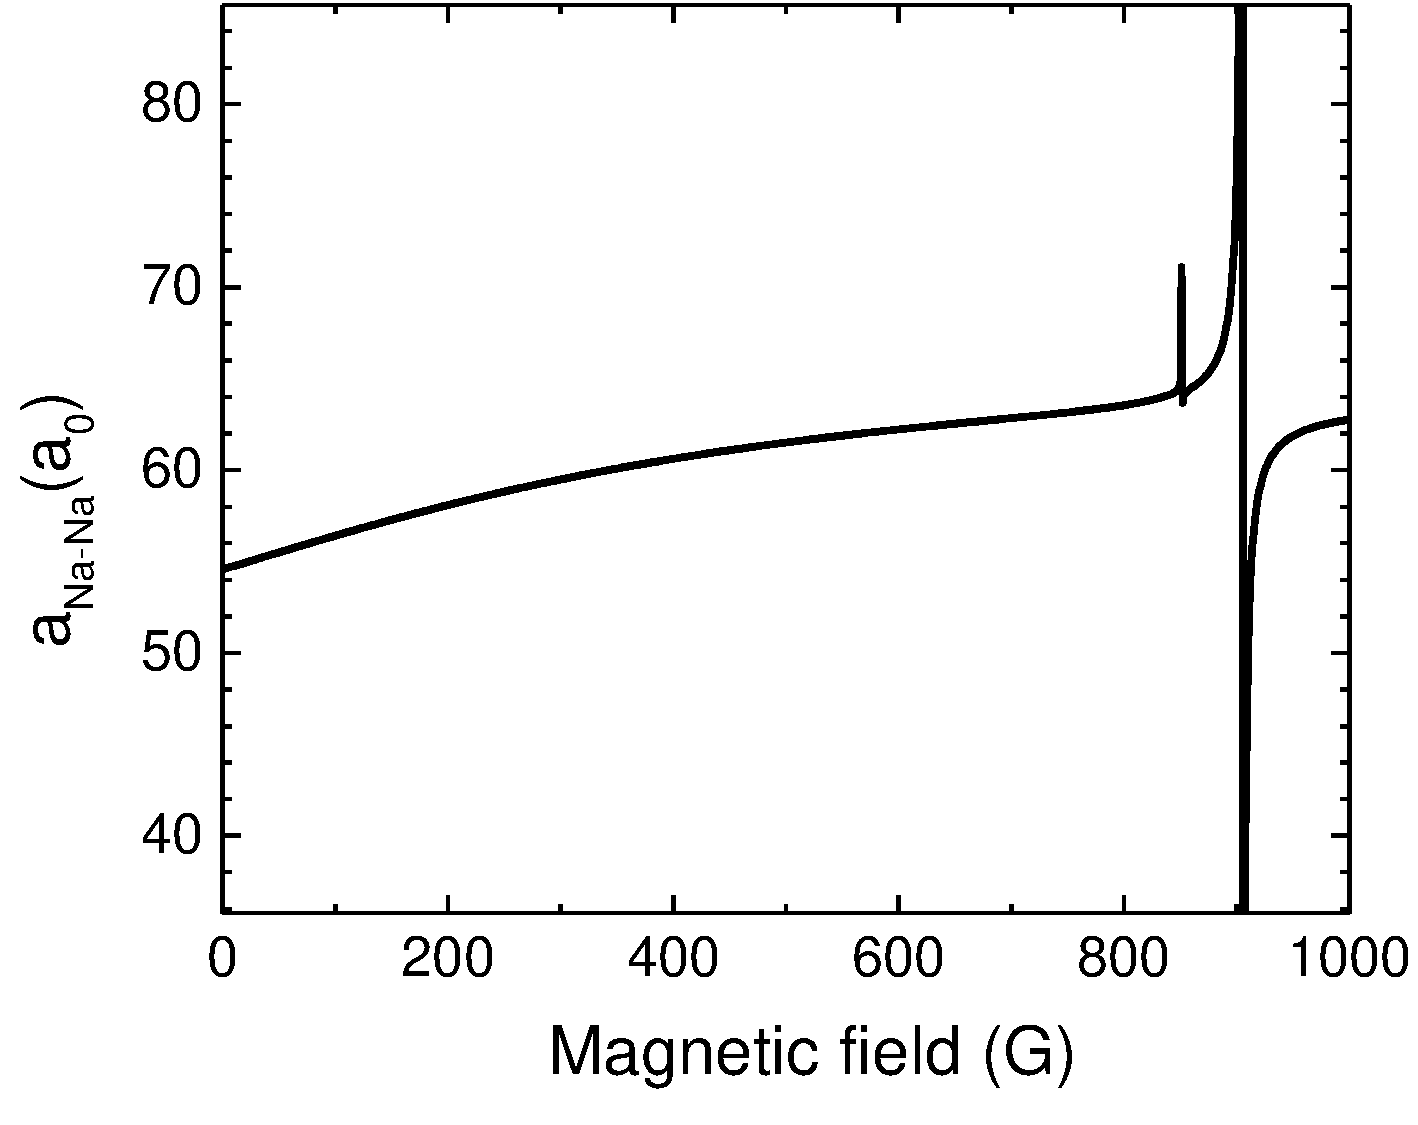
\includegraphics[width = \linewidth]{FR_NaNa.pdf}
\end{center}
\caption{}
\label{FR_NaNa}
\end{figure}